\chapter{Types, Variables and Assignment}
In this step , we will support data types and variables to SLANG. Assignment statement will also be implemented in this step.
The language supports only three data types viz.,\\
NUMERIC\\
STRING\\
BOOLEAN\\
\section{Type Info}
Let us add an Enum for data types
\lstset{style=csharp}
\begin{lstlisting}
// Type info enumerations
public enum TYPE_INFO
{
	TYPE_ILLEGAL = -1, // NOT A TYPE
	TYPE_NUMERIC, // IEEE Double precision floating point
	TYPE_BOOL, // Boolean Data type
	TYPE_STRING, // String data type
}
\end{lstlisting}

\section{Symbol Info}
Every variable will have a name, type and a slot for storing it's value in the symbol table.

Moreover, Functions return SYMBOL\_INFO.
\lstset{style=csharp}
\begin{lstlisting}
// Symbol Table entry for variable
// using Attributes , one can optimize the
// storage by simulating C/C++ union.
public class SYMBOL_INFO
{
	public String SymbolName; // Symbol Name
	public TYPE_INFO Type; // Data type
	public String str_val; // memory to hold string
	public double dbl_val; // memory to hold double
	public bool bol_val; // memory to hold boolean
}
\end{lstlisting}

\section{Exp}
The next step is to modify the Exp and Stmt interface to reflect the variable support.
\lstset{style=csharp}
\begin{lstlisting}
// In this Step , we add two more methods to the Exp class
// TypeCheck => To do Type analysis
// get_type => Type of this node
abstract class Exp
{
	public abstract 
	SYMBOL_INFO Evaluate(RUNTIME_CONTEXT cont);
	
	public abstract 
	TYPE_INFO TypeCheck(COMPILATION_CONTEXT cont);
	
	public abstract TYPE_INFO get_type();
}
\end{lstlisting}

\lstset{style=csharp}
\begin{lstlisting}
// 	Abstract base Class for Statement
public abstract class Stmt
{
	public abstract 
	SYMBOL_INFO Execute(RUNTIME_CONTEXT cont);     
}
\end{lstlisting}

\section{Contexts}
The classes RunTime context and CompileTime context contain the Symbol Table during interpretation.
\lstset{style=csharp}
\begin{lstlisting}
// A Context is necessary for Variable scope.
public class RUNTIME_CONTEXT
{
	// Symbol Table for this context
	private SymbolTable m_dt;
	
	// Create an instance of Symbol Table
	public RUNTIME_CONTEXT()
	{
		m_dt = new SymbolTable();
	}
	
	// Property to retrieve Table
	public SymbolTable TABLE
	{
		get => m_dt;
		set => m_dt = value;
	}
}

// A Context is necessary for Variable scope.
public class COMPILATION_CONTEXT
{
    /// Symbol Table for this context
    private SymbolTable m_dt = new SymbolTable();

    /// Property to retrieve Table
    public SymbolTable TABLE
    {
        get => m_dt;
        set => m_dt = value;
    }
}
\end{lstlisting}
\section{Constants}
Let us write the code for BooleanConstant node. This will store TRUE or FALSE value.
\lstset{style=csharp}
\begin{lstlisting}
// Node for Boolean Constant ( TRUE, FALSE }
public class BooleanConstant : Exp
{
	// Info Field
	private SYMBOL_INFO info;

	// Ctor
	public BooleanConstant(bool pvalue)
	{
		info = new SYMBOL_INFO();
		info.SymbolName = null;
		info.bol_val = pvalue;
		info.Type = TYPE_INFO.TYPE_BOOL;
	}

	// Evaluation of boolean will given the value
	public override SYMBOL_INFO Evaluate(RUNTIME_CONTEXT cont)
	{
		return info;
	}

	public override TYPE_INFO 
	TypeCheck(COMPILATION_CONTEXT cont)
	{
		return info.Type;
	}

	public override TYPE_INFO get_type()
	{
		return info.Type;
	}
}
\end{lstlisting}
The next thing which we should support is NumericConstant. This will store a IEEE 754 double precision floating point value.
\lstset{style=csharp}
\begin{lstlisting}
public class NumericConstant : Exp
{
	// Info field
	private SYMBOL_INFO info;
	public NumericConstant(double pvalue)
	{
		info = new SYMBOL_INFO();
		info.SymbolName = null;
		info.dbl_val = pvalue;
		info.Type = TYPE_INFO.TYPE_NUMERIC;
	}
		
	// Evaluation of boolean will given the value
	public override SYMBOL_INFO Evaluate(RUNTIME_CONTEXT cont)
	{
		return info;
	}
	
	public override TYPE_INFO 
	TypeCheck(COMPILATION_CONTEXT cont)
	{
		return info.Type;
	}
	
	public override TYPE_INFO get_type()
	{
		return info.Type;
	}
}
\end{lstlisting}
The AST node for storing String Literal is as given below.
\lstset{style=csharp}
\begin{lstlisting}
// To Store Literal string enclosed in quotes
public class StringLiteral : Exp
{
	// info field
	private SYMBOL_INFO info;

	public StringLiteral(string pvalue)
	{
		info = new SYMBOL_INFO();
		info.SymbolName = null;
		info.str_val = pvalue;
		info.Type = TYPE_INFO.TYPE_STRING;
	}

	public override SYMBOL_INFO Evaluate(RUNTIME_CONTEXT cont)
	{
		return info;
	}

	public override TYPE_INFO 
	TypeCheck(COMPILATION_CONTEXT cont)
	{
		return info.Type;
	}

	public override TYPE_INFO get_type()
	{
		return info.Type;
	}
}
\end{lstlisting}

\section{Variables}
Addding support to variable is an involved activity. The code has been extensively commented to explain the rationale.
\lstset{style=csharp}
\begin{lstlisting}

// Node to store Variables
// The data types supported are
// NUMERIC, STRING and BOOLEAN
// The node store only the variable name,
// the associated data will be found in the
// Symbol Table attached to the
// COMPILATION_CONTEXT
//
public class Variable : Exp
{
	private string m_name; // Var name
	TYPE_INFO _type; // Type

	public Variable(SYMBOL_INFO inf)
	{
		m_name = inf.SymbolName;
	}

	// Creates a new symbol and 
	// puts into the symbol table
	// and stores the key ( variable name )
	public Variable(COMPILATION_CONTEXT st, 
		String name, 
		double _value)
	{
		SYMBOL_INFO s = new SYMBOL_INFO();
		s.SymbolName = name;
		s.Type = TYPE_INFO.TYPE_NUMERIC;
		s.dbl_val = _value;
		st.TABLE.Add(s);
		m_name = name;
	}

	// Creates a new symbol and 
	// puts into the symbol table
	// and stores the key ( variable name )
	public Variable(COMPILATION_CONTEXT st, 
		String name, 
		bool _value)
	{
		SYMBOL_INFO s = new SYMBOL_INFO();
		s.SymbolName = name;
		s.Type = TYPE_INFO.TYPE_BOOL;
		s.bol_val = _value;
		st.TABLE.Add(s);
		m_name = name;
	}

	// Creates a new symbol and 
	// puts into the symbol table
	// and stores the key ( variable name )
	public Variable(COMPILATION_CONTEXT st, 
		String name, 
		string _value)
	{
		SYMBOL_INFO s = new SYMBOL_INFO();
		s.SymbolName = name;
		s.Type = TYPE_INFO.TYPE_STRING;
		s.str_val = _value;
		st.TABLE.Add(s);
		m_name = name;
	}

	// Retrieves the name of
	// the Variable ( method version )
	public string GetName()
	{
		return m_name;
	}

	// Retrieves the name of 
	// the Variable ( property version )
	public string Name
	{
		get { return m_name; }
		set { m_name = value; }
	}

	// To Evaluate a variable,  
	// we just need to do a lookup
	// in the Symbol table 
	// ( of RUNTIME_CONTEXT )
	public override SYMBOL_INFO Evaluate(RUNTIME_CONTEXT cont)
	{
		if (cont.TABLE == null)
		{
			return null;
		}
		else
		{
			SYMBOL_INFO a = cont.TABLE.Get(m_name);
			return a;
		}
	}

	// Look it up in the Symbol Table and
	// return the type
	public override TYPE_INFO 
	TypeCheck(COMPILATION_CONTEXT cont)
	{
		if (cont.TABLE == null)
		{
			return TYPE_INFO.TYPE_ILLEGAL;
		}
		else
		{
			SYMBOL_INFO a = cont.TABLE.Get(m_name);
			if (a != null)
			{
				_type = a.Type;
				return _type;
			}
			return TYPE_INFO.TYPE_ILLEGAL;
		}
	}

	// this should only be called after 
	// the TypeCheck method
	// has been invoked on AST
	public override TYPE_INFO get_type()
	{
		return _type;
	}
}
\end{lstlisting}


\clearpage
\section{Exp hierarchy}
At this point of time Expression hierarchy ( without operators ) looks like as follows.
\begin{verbatim}
Exp
    BooleanConstant
    NumericConstant
    StringLiteral
    Variable
\end{verbatim}

\section{Operators}
Once we have created nodes to represents constants of the type which we are planning to support, we created a variable node. The next challenge is to add support for the operators. Till now, I had UnaryExp and BinaryExp. For clarity, I will have classes like Plus ( + ), Minus (-), Div ( / ) and Mul (*) for BinaryExp and will have classes UnaryPlus ( + ), UnaryMinus ( -) for Unary operators.

\subsection{Binary Plus}
The first operator to be supported is Binary +

\lstset{style=csharp}
\begin{lstlisting}
// the node to represent Binary +
public class BinaryPlus : Exp
{

	// Plus has got a left expression (exp1 )
	// and a right expression...
	// and a Associated type information
	private Exp exp1, exp2;
	TYPE_INFO _type;
	public BinaryPlus(Exp e1, Exp e2)
	{
		exp1 = e1; 
		exp2 = e2;
	}

	public override SYMBOL_INFO Evaluate(RUNTIME_CONTEXT cont)
	{
		SYMBOL_INFO eval_left = exp1.Evaluate(cont);
		SYMBOL_INFO eval_right = exp2.Evaluate(cont);
		if (eval_left.Type == TYPE_INFO.TYPE_STRING &&
			eval_right.Type == TYPE_INFO.TYPE_STRING)
		{
			SYMBOL_INFO ret_val = new SYMBOL_INFO();
			ret_val.str_val = eval_left.str_val 
								+ eval_right.str_val;
			ret_val.Type = TYPE_INFO.TYPE_STRING;
			ret_val.SymbolName = "";
			return ret_val;
		}
		else if 
		(eval_left.Type == TYPE_INFO.TYPE_NUMERIC &&
		eval_right.Type == TYPE_INFO.TYPE_NUMERIC)
		{
			SYMBOL_INFO ret_val = new SYMBOL_INFO();
			ret_val.dbl_val = 
				eval_left.dbl_val + eval_right.dbl_val;
			ret_val.Type = TYPE_INFO.TYPE_NUMERIC;
			ret_val.SymbolName = "";
			return ret_val;
		}
		else {
			throw new Exception("Type mismatch");
		}
	}
	
	public override TYPE_INFO 
	TypeCheck(COMPILATION_CONTEXT cont)
	{
		TYPE_INFO eval_left = exp1.TypeCheck(cont);
		TYPE_INFO eval_right = exp2.TypeCheck(cont);
		if (eval_left == eval_right && 
		eval_left != TYPE_INFO.TYPE_BOOL)
		{
			_type = eval_left;
			return _type;
		}
		else {
			throw new Exception("Type mismatch failure");
		}
	}
	
	public override TYPE_INFO get_type()
	{
		return _type;
	}
}
\end{lstlisting}

Where as Evaluate routine for StringLiteral , NumericConstant , BooleanConstant and Variable just
involves returning the SYMBOL\_INO , in the case of Operators things are bit evolved...

\lstset{style=csharp}
\begin{lstlisting}
public override SYMBOL_INFO Evaluate(RUNTIME_CONTEXT cont)
{
	SYMBOL_INFO eval_left = exp1.Evaluate(cont);
	SYMBOL_INFO eval_right = exp2.Evaluate(cont);
	if (eval_left.Type == TYPE_INFO.TYPE_STRING &&
		eval_right.Type == TYPE_INFO.TYPE_STRING)
	{
		SYMBOL_INFO ret_val = new SYMBOL_INFO();
		ret_val.str_val = 
			eval_left.str_val + eval_right.str_val;
		ret_val.Type = TYPE_INFO.TYPE_STRING;
		ret_val.SymbolName = "";
		return ret_val;
	}
	else if (eval_left.Type == TYPE_INFO.TYPE_NUMERIC &&
			eval_right.Type == TYPE_INFO.TYPE_NUMERIC)
	{
		SYMBOL_INFO ret_val = new SYMBOL_INFO();
		ret_val.dbl_val = eval_left.dbl_val 
							+ eval_right.dbl_val;
		ret_val.Type = TYPE_INFO.TYPE_NUMERIC;
		ret_val.SymbolName = "";
		return ret_val;
	}
	else {
		throw new Exception("Type mismatch");
	}
}
\end{lstlisting}

In the above code snippet , Left and Right expressions are evaluated and the types are queried. In our compiler , operations involving numerics and strings are successful only if all the operands are of the same type.

The routine TypeCheck is similar to Evaluate. Only difference is that TypeCheck updates the type information of the nodes in a Recursive manner. The routine get\_type is only valid once you have called TypeCheck routine.

\subsection{Binary Minus}
BinaryMinus is similar to BinaryPlus. The only difference is only Numerics can be subtracted.


\lstset{style=csharp}
\begin{lstlisting}
class BinaryMinus : Exp
{
	private Exp exp1, exp2;
	TYPE_INFO _type;
	public BinaryMinus(Exp e1, Exp e2)
	{
		exp1 = e1; 
		exp2 = e2;
	}
	public override SYMBOL_INFO Evaluate(RUNTIME_CONTEXT cont)
	{
		SYMBOL_INFO eval_left = exp1.Evaluate(cont);
		SYMBOL_INFO eval_right = exp2.Evaluate(cont);
		if (eval_left.Type == TYPE_INFO.TYPE_NUMERIC &&
			eval_right.Type == TYPE_INFO.TYPE_NUMERIC)
		{
			SYMBOL_INFO ret_val = new SYMBOL_INFO();
			ret_val.dbl_val = eval_left.dbl_val 
								- eval_right.dbl_val;
			ret_val.Type = TYPE_INFO.TYPE_NUMERIC;
			ret_val.SymbolName = "";
			return ret_val;
		}
		else {
			throw new Exception("Type mismatch");
		}
	}
	
	public override TYPE_INFO 
	TypeCheck(COMPILATION_CONTEXT cont)
	{
		TYPE_INFO eval_left = exp1.TypeCheck(cont);
		TYPE_INFO eval_right = exp2.TypeCheck(cont);
		if (eval_left == eval_right && 
			eval_left == TYPE_INFO.TYPE_NUMERIC)
		{
			_type = eval_left;
			return _type;
		}
		else{
			throw new Exception("Type mismatch failure");
		}
	}

	public override TYPE_INFO get_type()
	{
		return _type;
	}
}
\end{lstlisting}

\subsection{Mul and Div}
Multiplication and Division operators are only valid for Numeric Types. If you have understood the
implementation of BinaryPlus , the Mul and Div operators are easy to follow.


\lstset{style=csharp}
\begin{lstlisting}
\\Mul Node
class Mul : Exp
{
	private Exp exp1, exp2;
	TYPE_INFO _type;
	public Mul(Exp e1, Exp e2)
	{
		exp1 = e1; 
		exp2 = e2;
	}
	
	public override SYMBOL_INFO Evaluate(RUNTIME_CONTEXT cont)
	{
		SYMBOL_INFO eval_left = exp1.Evaluate(cont);
		SYMBOL_INFO eval_right = exp2.Evaluate(cont);
		if (eval_left.Type == TYPE_INFO.TYPE_NUMERIC &&
			eval_right.Type == TYPE_INFO.TYPE_NUMERIC)
		{
			SYMBOL_INFO ret_val = new SYMBOL_INFO();
			ret_val.dbl_val = eval_left.dbl_val 
								* eval_right.dbl_val;
			ret_val.Type = TYPE_INFO.TYPE_NUMERIC;
			ret_val.SymbolName = "";
			return ret_val;
		}
		else {
			throw new Exception("Type mismatch");
		}
	}
	
	public override TYPE_INFO 
	TypeCheck(COMPILATION_CONTEXT cont)
	{
		TYPE_INFO eval_left = exp1.TypeCheck(cont);
		TYPE_INFO eval_right = exp2.TypeCheck(cont);
		if (eval_left == eval_right && 
		eval_left == TYPE_INFO.TYPE_NUMERIC)
		{
			_type = eval_left;
			return _type;
		}
		else {
			throw new Exception("Type mismatch failure");
		}
	}
	
	public override TYPE_INFO get_type()
	{
		return _type;
	}
}

//Div Node
class Div : Exp
{
	private Exp exp1, exp2;
	TYPE_INFO _type;
	public Div(Exp e1, Exp e2)
	{
		exp1 = e1; 
		exp2 = e2;
	}

	public override SYMBOL_INFO Evaluate(RUNTIME_CONTEXT cont)
	{
		SYMBOL_INFO eval_left = exp1.Evaluate(cont);
		SYMBOL_INFO eval_right = exp2.Evaluate(cont);
		if (eval_left.Type == TYPE_INFO.TYPE_NUMERIC &&
		eval_right.Type == TYPE_INFO.TYPE_NUMERIC)
		{
			SYMBOL_INFO ret_val = new SYMBOL_INFO();
			ret_val.dbl_val = eval_left.dbl_val 
								/ eval_right.dbl_val;
			ret_val.Type = TYPE_INFO.TYPE_NUMERIC;
			ret_val.SymbolName = "";
			return ret_val;
		}
		else
		{
			throw new Exception("Type mismatch");
		}
	}

	public override TYPE_INFO 
	TypeCheck(COMPILATION_CONTEXT cont)
	{
		TYPE_INFO eval_left = exp1.TypeCheck(cont);
		TYPE_INFO eval_right = exp2.TypeCheck(cont);
		if (eval_left == eval_right && 
			eval_left == TYPE_INFO.TYPE_NUMERIC)
		{
			_type = eval_left;
			return _type;
		}
		else {
			throw new Exception("Type mismatch failure");
		}
	}
	
	public override TYPE_INFO get_type()
	{
		return _type;
	}
}
\end{lstlisting}

\subsection{Unary Plus and Unary Minus}
UnaryPlus and UnaryMinus is also similar to the implementation of other operators. Both these operators are only applicable for Numeric data type.
\lstset{style=csharp}
\begin{lstlisting}
// the node to represent Unary +
class UnaryPlus : Exp
{
	// Plus has got a right expression (exp1 )
	// and a Associated type information
	private Exp exp1;
	TYPE_INFO _type;
	public UnaryPlus(Exp e1)
	{
		exp1 = e1;
	}
	
	public override SYMBOL_INFO Evaluate(RUNTIME_CONTEXT cont)
	{
		SYMBOL_INFO 
		eval_left = exp1.Evaluate(cont);
		if (eval_left.Type == TYPE_INFO.TYPE_NUMERIC)
		{
			SYMBOL_INFO ret_val = new SYMBOL_INFO();
			ret_val.dbl_val = eval_left.dbl_val;
			ret_val.Type = TYPE_INFO.TYPE_NUMERIC;
			ret_val.SymbolName = "";
			return ret_val;
		}
		else {
			throw new Exception("Type mismatch");
		}
	}
	
	public override TYPE_INFO 
	TypeCheck(COMPILATION_CONTEXT cont)
	{
		TYPE_INFO eval_left = exp1.TypeCheck(cont);
		if (eval_left == TYPE_INFO.TYPE_NUMERIC)
		{
			_type = eval_left;
			return _type;
		}
		else {
			throw new Exception("Type mismatch failure");
		}
	}
	
	public override TYPE_INFO get_type()
	{
		return _type;
	}
}

// the node to represent Unary -
class UnaryMinus : Exp
{
	// Plus has got a right expression (exp1 )
	// and a Associated type information
	private Exp exp1;
	TYPE_INFO _type;
	public UnaryMinus(Exp e1)
	{
		exp1 = e1;
	}
	
	public override SYMBOL_INFO Evaluate(RUNTIME_CONTEXT cont)
	{
		SYMBOL_INFO 
		eval_left = exp1.Evaluate(cont);
		if (eval_left.Type == TYPE_INFO.TYPE_NUMERIC)
		{
			SYMBOL_INFO ret_val = new SYMBOL_INFO();
			ret_val.dbl_val = -eval_left.dbl_val;
			ret_val.Type = TYPE_INFO.TYPE_NUMERIC;
			ret_val.SymbolName = "";
			return ret_val;
		}
		else {
			throw new Exception("Type mismatch");
		}
	}
	
	public override TYPE_INFO 
	TypeCheck(COMPILATION_CONTEXT cont)
	{
		TYPE_INFO eval_left = exp1.TypeCheck(cont);
		if (eval_left == TYPE_INFO.TYPE_NUMERIC)
		{
			_type = eval_left;
			return _type;
		}
		else {
			throw new Exception("Type mismatch failure");
		}
	}

	public override TYPE_INFO get_type()
	{
		return _type;
	}
}
\end{lstlisting}

\section{Statements}
The statement related nodes are moved to a seperate module by the name AstForStatements. In this step , we have added support for Variable Declaration and Assignment statement. 
\subsection{Variable Declaration}
The AST for Variable declaration is given below.
\lstset{style=csharp}
\begin{lstlisting}
// Compile the Variable Declaration statements
public class VariableDeclStatement : Stmt
{
	SYMBOL_INFO m_inf = null;
	Variable var = null;
	
	public VariableDeclStatement(SYMBOL_INFO inf)
	{
		m_inf = inf;
	}
	
	public override SYMBOL_INFO Execute(RUNTIME_CONTEXT cont)
	{
		cont.TABLE.Add(m_inf);
		var = new Variable(m_inf);
		return null;
	}
}
\end{lstlisting}
In the parser, before we create VariableDeclStatement node, we need to insert the variable's SYMBOL\_INFO into the SymbolTable of the COMPILATION\_CONTEXT. The VariableDeclStatement node just stores the variable name in the Variable AST. While Executing the VariableDeclStatement, a Variable is created in the Symbol table of RUNTIME\_CONTEXT. Both Compilation Context ( COMPILATION\_CONTEXT ) and Run time Context ( RUNTIME\_CONTEXT ) just contains references to respective symbol tables. 
\clearpage
\subsection{Assignment}
The AST for Assignment statement is given below.
\lstset{style=csharp}
\begin{lstlisting}
// Assignment Statement
public class AssignmentStatement : Stmt
{
	private Variable variable;
	private Exp exp1;
	public AssignmentStatement(Variable var, Exp e)
	{
		variable = var;
		exp1 = e;
	}
	
	public AssignmentStatement(SYMBOL_INFO var, Exp e)
	{
		variable = new Variable(var);
		exp1 = e;
	}
	
	public override SYMBOL_INFO Execute(RUNTIME_CONTEXT cont)
	{
		SYMBOL_INFO val = exp1.Evaluate(cont);
		cont.TABLE.Assign(variable, val);
		return null;
	}
}
\end{lstlisting}
\clearpage
\subsection{AST for statements}
At this point of time, AST for Statements is as shown below.
\begin{verbatim}
class Stmt
	class VariableDeclStatement
	class AssignmentStatement
	class PrintStatement
	class PrintLineStatement
\end{verbatim}

\section{Symbol Table}
The class SymbolTable is just a vector of name-value pair . The source code of the SymbolTable is given below.

\lstset{style=csharp}
\begin{lstlisting}
// Symbol Table for Parsing and Type Analysis
public class SymbolTable
{
	// private data structure
	private System.Collections.Hashtable dt = new Hashtable();

	// Add a symbol to Symbol Table
	public bool Add(SYMBOL_INFO s)
	{
		dt[s.SymbolName] = s;
		return true;
	}

	// Retrieve the Symbol
	public SYMBOL_INFO Get(string name)
	{
		return dt[name] as SYMBOL_INFO;
	}

	// Assign to the Symbol Table
	public void Assign(Variable var, SYMBOL_INFO value)
	{
		value.SymbolName = var.GetName();
		dt[var.GetName()] = value;
	}

	// Assign to a variable
	public void Assign(string var, SYMBOL_INFO value)
	{
		dt[var] = value;
	}
}
\end{lstlisting}
\section{Support classes}
The class CsyntaxErrorLog and CsemanticErrorLog ( in SupportClasses.cs ) is meant for error logging
while the compilation process is going on.....
\section{Lexical Analysis}
Let us go back to Lexical Analysis stage once again. This time we have added lot of new keywords to the language and Token set has become bit larger than the previous step.
\subsection{Tokens}
\lstset{style=csharp}
\begin{lstlisting}
public enum TOKEN
{
	ILLEGAL_TOKEN = -1, // Not a Token
	TOK_PLUS = 1, // '+'
	TOK_MUL, // '*'
	TOK_DIV, // '/'
	TOK_SUB, // '-'
	TOK_OPAREN, // '('
	TOK_CPAREN, // ')'
	TOK_NULL, // End of string
	TOK_PRINT, // Print Statement
	TOK_PRINTLN, // PrintLine
	TOK_UNQUOTED_STRING, // Variable name , Function name etc
	TOK_SEMI , // ;
	//---------- Addition in Step 4
	TOK_VAR_NUMBER, // NUMBER data type
	TOK_VAR_STRING, // STRING data type
	TOK_VAR_BOOL, // Bool data type
	TOK_NUMERIC, // [0-9]+
	TOK_COMMENT , // Comment Token ( presently not used )
	TOK_BOOL_TRUE, // Boolean TRUE
	TOK_BOOL_FALSE , // Boolean FALSE
	TOK_STRING, // String Literal
	TOK_ASSIGN // Assignment Symbol =
}
\end{lstlisting}
\subsection{Additions}
We have also moved couple of routines and state variables to Lexer class. The two notable addition are:
\lstset{style=csharp}
\begin{lstlisting}
// Current Token and Last Grabbed Token
protected TOKEN Current_Token; // Current Token
protected TOKEN Last_Token; // Penultimate token
\end{lstlisting}
Since we have added support for string type..., we need to support string literals (or the last grabbed string) in the lexical analyzer...
\lstset{style=csharp}
\begin{lstlisting}
public String last_str; // Last grabbed String
\end{lstlisting}
We need to update the keyword table with additional key words supported by the compiler.
\lstset{style=csharp}
\begin{lstlisting}
// Fill the Keywords
keyword = new ValueTable[7];
keyword[0] = new ValueTable(TOKEN.TOK_BOOL_FALSE, "FALSE");
keyword[1] = new ValueTable(TOKEN.TOK_BOOL_TRUE, "TRUE");
keyword[2] = new ValueTable(TOKEN.TOK_VAR_STRING, "STRING");
keyword[3] = new ValueTable(TOKEN.TOK_VAR_BOOL, "BOOLEAN");
keyword[4] = new ValueTable(TOKEN.TOK_VAR_NUMBER, "NUMERIC");
keyword[5] = new ValueTable(TOKEN.TOK_PRINT, "PRINT");
keyword[6] = new ValueTable(TOKEN.TOK_PRINTLN, "PRINTLINE");
\end{lstlisting}
\section{Parsing}
\subsection{Parser Entrypoint}
The Parsing of the statements starts from Parse Routine of RDParser.cs
\lstset{style=csharp}
\begin{lstlisting}
// The new Parser entry point
public ArrayList Parse(COMPILATION_CONTEXT ctx)
{
	GetNext(); // Get the Next Token
	// Parse all the statements
	return StatementList(ctx);
}
\end{lstlisting}
Any variable encountered during the Parse Process will be put into the symbol table associated with COMPILATION\_CONTEXT
\subsection{Statement List}
The Logic of the StatementList is as follows,
\begin{verbatim}
while there is more statements
	Parse and Add Statements to the ArrayList
\end{verbatim}


\lstset{style=csharp}
\begin{lstlisting}
private ArrayList StatementList(COMPILATION_CONTEXT ctx)
{
	ArrayList arr = new ArrayList();
	while (Current_Token != TOKEN.TOK_NULL)
	{
		Stmt temp = Statement(ctx);
		if (temp != null)
		{
			arr.Add(temp);
		}
	}
	return arr;
}
\end{lstlisting}

\subsection{Grammar}
The Grammar supported is given below
\lstset{style=csharp}
\begin{lstlisting}
<stmtlist> := { <statement> }+
{<statement> := <printstmt> | <printlinestmt>
<printstmt> := print <expr >;
<vardeclstmt> := 
STRING <varname>; |
NUMERIC <varname>; |
BOOLEAN <varname>;
<printlinestmt>:= printline <expr>;
<Expr> ::= <Term> | <Term> { + | - } <Expr>
<Term> ::= <Factor> | <Factor> {*|/} <Term>
<Factor>::= <number> | ( <expr> ) | {+|-} <factor> |
<variable> | TRUE | FALSE
\end{lstlisting}

\subsection{Statement}
The Statement method just queries the statement type and calls the appropriate Parse Routines.
\lstset{style=csharp}
\begin{lstlisting}
// This Routine Queries Statement Type
// to take the appropriate Branch...
// Currently , only Print and PrintLine statement
// are supported..
// if a line does not start with Print or PrintLine ..
// an exception is thrown
private Stmt Statement(COMPILATION_CONTEXT ctx)
{
	Stmt retval = null;
	switch (Current_Token)
	{
		case TOKEN.TOK_VAR_STRING:
		case TOKEN.TOK_VAR_NUMBER:
		case TOKEN.TOK_VAR_BOOL:
			retval = 
				ParseVariableStatement(ctx);
			GetNext();
			return retval;
		
		case TOKEN.TOK_PRINT:
			retval = ParsePrintStatement(ctx);
			GetNext();
			break;
		
		case TOKEN.TOK_PRINTLN:
			retval = ParsePrintLNStatement(ctx);
			GetNext();
			break;

		case TOKEN.TOK_UNQUOTED_STRING:
			retval = ParseAssignmentStatement(ctx);
			GetNext();
			return retval;
		
		default:
			throw new Exception("Invalid statement");
	}
	return retval;
}
\end{lstlisting}

\subsection{ParseVariableDeclStatement}
The Source code of the ParseVariableDeclStatement is as given below.
\lstset{style=csharp}
\begin{lstlisting}
// Parse Variable declaration statement
public Stmt 
ParseVariableDeclStatement(COMPILATION_CONTEXT ctx)
{
	//--- Save the Data type
	TOKEN tok = Current_Token;
	// --- Skip to the next token , the token ought
	// to be a Variable name ( UnQouted String )
	GetNext();
	if (Current_Token == TOKEN.TOK_UNQUOTED_STRING)
	{
		SYMBOL_INFO symb = new SYMBOL_INFO();
		symb.SymbolName = base.last_str;
		symb.Type = (tok == TOKEN.TOK_VAR_BOOL) ?
		TYPE_INFO.TYPE_BOOL : 
			(tok == TOKEN.TOK_VAR_NUMBER) ?
		TYPE_INFO.TYPE_NUMERIC : TYPE_INFO.TYPE_STRING;
		//---------- Skip to Expect the SemiColon
		GetNext();
		if (Current_Token == TOKEN.TOK_SEMI)
		{
			// ----------- Add to the Symbol Table
			// for type analysis
			ctx.TABLE.Add(symb);
			// --------- return the Object of type
			// --------- VariableDeclStatement
			// This will just store the Variable name
			// to be looked up in the above table
			return new VariableDeclStatement(symb);
		}
		else
		{
			CSyntaxErrorLog.AddLine("; expected");
			CSyntaxErrorLog.AddLine(GetCurrentLine(SaveIndex()));
			throw 
			new CParserException(-100, ", or ; expected", SaveIndex());
		}
	}
	else
	{
		CSyntaxErrorLog.AddLine("invalid variable declaration");
		CSyntaxErrorLog.AddLine(GetCurrentLine(SaveIndex()));
		throw  
		new CParserException(-100, ", or ; expected", SaveIndex());
	}
}
\end{lstlisting}
\subsection{AssignmentStatement}
Assignment statement is easy to parse as the required ground work has already been done... !
\lstset{style=csharp}
\begin{lstlisting}
// Parse the Assignment Statement
public Stmt ParseAssignmentStatement(COMPILATION_CONTEXT ctx)
{
	// Retrieve the variable and look it up in
	// the symbol table ..if not found throw exception
	string variable = base.last_str;
	SYMBOL_INFO s = ctx.TABLE.Get(variable);
	if (s == null)
	{
		CSyntaxErrorLog.AddLine("Variable not found " + last_str);
		CSyntaxErrorLog.AddLine(GetCurrentLine(SaveIndex()));
		throw 
		new CParserException(-100, "Variable not found", SaveIndex());
	}
 
	//------------ The next token ought to be an assignment
	// expression....
	GetNext();
	if (Current_Token != TOKEN.TOK_ASSIGN)
	{
		CSyntaxErrorLog.AddLine("= expected");
		CSyntaxErrorLog.AddLine(GetCurrentLine(SaveIndex()));
		throw 
		new CParserException(-100, "= expected", SaveIndex());
	}
	//-------- Skip the token to start the expression
	// parsing on the RHS
	GetNext();
	Exp exp = Expr(ctx);
	//------------ Do the type analysis ...
	if (exp.TypeCheck(ctx) != s.Type)
	{
		throw new Exception("Type mismatch in assignment");
	}
	// -------------- End of statement ( ; ) is expected
	if (Current_Token != TOKEN.TOK_SEMI)
	{
		CSyntaxErrorLog.AddLine("; expected");
		CSyntaxErrorLog.AddLine(GetCurrentLine(SaveIndex()));
		throw new CParserException(-100, " ; expected", -1);
	}
	// return an instance of AssignmentStatement node..
	// s => Symbol info associated with variable
	// exp => to evaluated and assigned to symbol_info
	return new AssignmentStatement(s, exp);
}
\end{lstlisting}
\subsection{Parsing Expressions}
\subsubsection{Grammar for Expression}
The grammar for expression is given below.
\lstset{style=csharp}
\begin{lstlisting}
<Expr> ::= <Term> | <Term> { + | - } <Expr>
<Term> ::= <Factor> | <Factor> {*|/} <Term>
<Factor>::= <number> | ( <expr> ) | {+|-} <factor>
<variable> | TRUE | FALSE
\end{lstlisting}
\subsubsection{Expression Routine}
Let us take a look at the Expression routine , ie the top most expression parsing routine at this point of time... ( In future , when logical expressions and relational expressions are added , we modify the grammar)
\lstset{style=csharp}
\begin{lstlisting}
/// <Expr> ::= <Term> | <Term> { + | - } <Expr>
public Exp Expr(COMPILATION_CONTEXT ctx)
{
	TOKEN l_token;
	Exp RetValue = Term(ctx);
	while (Current_Token == TOKEN.TOK_PLUS || 
		Current_Token == TOKEN.TOK_SUB)
	{
		l_token = Current_Token;
		Current_Token = GetToken();
		Exp e1 = Expr(ctx);
		if (l_token == TOKEN.TOK_PLUS)
			RetValue = new BinaryPlus(RetValue, e1);
		else
			RetValue = new BinaryMinus(RetValue, e1);
	}
	return RetValue;
}
\end{lstlisting}
\subsubsection{Term Routine}
The Term routine handles the mul and the div operators. 
\lstset{style=csharp}
\begin{lstlisting}
// <Term> ::= <Factor> | <Factor> {*|/} <Term>
public Exp Term(COMPILATION_CONTEXT ctx)
{
	TOKEN l_token;
	Exp RetValue = Factor(ctx);
	while (Current_Token == TOKEN.TOK_MUL || 
		Current_Token == TOKEN.TOK_DIV)
	{
		l_token = Current_Token;
		Current_Token = GetToken();
		Exp e1 = Term(ctx);
		if (l_token == TOKEN.TOK_MUL)
			RetValue = new Mul(RetValue, e1);
		else
			RetValue = new Div(RetValue, e1);
	}
	return RetValue;
}
\end{lstlisting}
\subsubsection{Factor Routine}
The factor routine is where we handle Variables , unary Operations , Constants etc....
\lstset{style=csharp}
\begin{lstlisting}
// <Factor>::= <number> | ( <expr> ) | {+|-} <factor> |
// <variable> | TRUE | FALSE
public Exp Factor(COMPILATION_CONTEXT ctx)
{
	TOKEN l_token;
	Exp RetValue = null;
	if (Current_Token == TOKEN.TOK_NUMERIC)
	{
		RetValue = new NumericConstant(GetNumber());
		Current_Token = GetToken();
	}
	else if (Current_Token == TOKEN.TOK_STRING)
	{
		RetValue = new StringLiteral(last_str);
		Current_Token = GetToken();
	}
	else if (Current_Token == TOKEN.TOK_BOOL_FALSE ||
		Current_Token == TOKEN.TOK_BOOL_TRUE)
	{
		RetValue = new BooleanConstant(
		Current_Token == 
			TOKEN.TOK_BOOL_TRUE ? true : false);
		Current_Token = GetToken();
	}
	else if (Current_Token == TOKEN.TOK_OPAREN)
	{
		Current_Token = GetToken();
		RetValue = Expr(ctx); // Recurse
		if (Current_Token != TOKEN.TOK_CPAREN)
		{
			Console.WriteLine("Missing Closing Parenthesis\n");
			throw new Exception();
		}
		Current_Token = GetToken();
	}
	else if (Current_Token == TOKEN.TOK_PLUS || 
		Current_Token == TOKEN.TOK_SUB)
	{
		l_token = Current_Token;
		Current_Token = GetToken();
		RetValue = Factor(ctx);
		if (l_token == TOKEN.TOK_PLUS)
			RetValue = new UnaryPlus(RetValue);
		else
			RetValue = new UnaryMinus(RetValue);
	}
	else if (Current_Token == TOKEN.TOK_UNQUOTED_STRING)
	{
		
		// Variables
		String str = base.last_str;
		SYMBOL_INFO inf = ctx.TABLE.Get(str);
		if (inf == null) {
			throw new Exception("Undefined symbol");
		}
		GetNext();
		RetValue = new Variable(inf);
	}
	else
	{
		Console.WriteLine("Illegal Token");
		throw new Exception();
	}
	return RetValue;
}
\end{lstlisting}
\section{Main}
In the CallSlang Project, this is how we need to invoke the Script....
\lstset{style=csharp}
\begin{lstlisting}
using System;
using System.Collections.Generic;
using System.Linq;
using System.Text;
using System.Collections;
using System.IO;
using SLANG_DOT_NET;
namespace CallSLANG
{
	class Program
	{
		// Driver routine to call the program script
		static void TestFileScript(string filename)
		{
			if (filename == null)
				return;
			
			//Read the contents from the file
			StreamReader sr = new StreamReader(filename);
			string programs2 = sr.ReadToEnd();
			
			//Creates the Parser Object
			// With Program text as argument
			RDParser pars = null;
			pars = new RDParser(programs2);

			// Create a Compilation Context
			COMPILATION_CONTEXT ctx = 
			new COMPILATION_CONTEXT();

			// Call the top level Parsing Routine with
			// Compilation Context as the Argument
			ArrayList stmts = pars.Parse(ctx);
			
			// if we have reached here , the parse process
			// is successful... Create a Run time context and
			// Call Execute statements of each statement...
			RUNTIME_CONTEXT f = new RUNTIME_CONTEXT();
			foreach(Object obj in stmts )
			{
				Stmt s = obj as Stmt;
				s.Execute(f);
			}
		}
		
		static void Main(string[] args)
		{
			if (args == null ||
				args.Length != 1)
			{
				Console.WriteLine(
					"CallSlang <scriptname>\n");
				return;
			}
			TestFileScript(args[0]);
			
			//Wait for the Key Press
			Console.Read();
		}
	} 
}
\end{lstlisting}
\section{SLANG scripts}
First.sl
\lstset{style=csharp}
\begin{lstlisting}
//First.sl ( Slang script )
NUMERIC a; // Declare a Numeric variable
a = 2*3+5* 30 + -(4*5+3); // Assign
PRINTLINE a; // Dump a

//String concatenation
PRINT "Hello " + "World";

//Write a new line
PRINTLINE "";

//string data type
STRING c;
c = "Hello "; // assignment to string

//assignment and concatenation
C = C + "World";
PRINTLINE c;

//boolean variable
BOOLEAN d;
d = TRUE;
PRINTLINE d;
d = FALSE;
PRINTLINE d;
\end{lstlisting}
Second.sl
\lstset{style=csharp}
\begin{lstlisting}
//Second.sl
// A slang script to test unary expression
Numeric a ;
a = -1 ;
a = -a;
Print a;
\end{lstlisting}
Third.sl
\lstset{style=csharp}
\begin{lstlisting}
Numeric a;
String b;
a = ---1;
PrintLine a*4 + 10;
\end{lstlisting}
You can go to the command line and invoke the CallSlang executable as follows....a screen snapshot is also given.\\
\begin{verbatim}
	CallSlang First.sl
	CallSlang Second.sl
	CallSlang Third.sl
\end{verbatim}
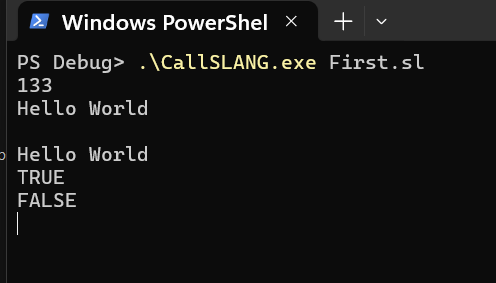
\includegraphics[width=0.5\textwidth]{first.png}
